\documentclass[journal,12pt,twocolumn]{IEEEtran}

\usepackage{setspace}
\usepackage{gensymb}
\singlespacing
\usepackage[cmex10]{amsmath}

\usepackage{amsthm}

\usepackage{mathrsfs}
\usepackage{txfonts}
\usepackage{stfloats}
\usepackage{bm}
\usepackage{cite}
\usepackage{cases}
\usepackage{subfig}

\usepackage{longtable}
\usepackage{multirow}

\usepackage{enumitem}
\usepackage{mathtools}
\usepackage{steinmetz}
\usepackage{tikz}
\usepackage{circuitikz}
\usepackage{verbatim}
\usepackage{tfrupee}
\usepackage[breaklinks=true]{hyperref}
\usepackage{graphicx}
\usepackage{tkz-euclide}

\usetikzlibrary{calc,math}
\usepackage{listings}
    \usepackage{color}                                            %%
    \usepackage{array}                                            %%
    \usepackage{longtable}                                        %%
    \usepackage{calc}                                             %%
    \usepackage{multirow}                                         %%
    \usepackage{hhline}                                           %%
    \usepackage{ifthen}                                           %%
    \usepackage{lscape}     
\usepackage{multicol}
\usepackage{chngcntr}

\DeclareMathOperator*{\Res}{Res}

\renewcommand\thesection{\arabic{section}}
\renewcommand\thesubsection{\thesection.\arabic{subsection}}
\renewcommand\thesubsubsection{\thesubsection.\arabic{subsubsection}}

\renewcommand\thesectiondis{\arabic{section}}
\renewcommand\thesubsectiondis{\thesectiondis.\arabic{subsection}}
\renewcommand\thesubsubsectiondis{\thesubsectiondis.\arabic{subsubsection}}


\hyphenation{op-tical net-works semi-conduc-tor}
\def\inputGnumericTable{}                                 %%

\lstset{
%language=C,
frame=single, 
breaklines=true,
columns=fullflexible
}
\begin{document}


\newtheorem{theorem}{Theorem}[section]
\newtheorem{problem}{Problem}
\newtheorem{proposition}{Proposition}[section]
\newtheorem{lemma}{Lemma}[section]
\newtheorem{corollary}[theorem]{Corollary}
\newtheorem{example}{Example}[section]
\newtheorem{definition}[problem]{Definition}

\newcommand{\BEQA}{\begin{eqnarray}}
\newcommand{\EEQA}{\end{eqnarray}}
\newcommand{\define}{\stackrel{\triangle}{=}}
\bibliographystyle{IEEEtran}
\raggedbottom
\setlength{\parindent}{0pt}
\providecommand{\mbf}{\mathbf}
\providecommand{\pr}[1]{\ensuremath{\Pr\left(#1\right)}}
\providecommand{\qfunc}[1]{\ensuremath{Q\left(#1\right)}}
\providecommand{\sbrak}[1]{\ensuremath{{}\left[#1\right]}}
\providecommand{\lsbrak}[1]{\ensuremath{{}\left[#1\right.}}
\providecommand{\rsbrak}[1]{\ensuremath{{}\left.#1\right]}}
\providecommand{\brak}[1]{\ensuremath{\left(#1\right)}}
\providecommand{\lbrak}[1]{\ensuremath{\left(#1\right.}}
\providecommand{\rbrak}[1]{\ensuremath{\left.#1\right)}}
\providecommand{\cbrak}[1]{\ensuremath{\left\{#1\right\}}}
\providecommand{\lcbrak}[1]{\ensuremath{\left\{#1\right.}}
\providecommand{\rcbrak}[1]{\ensuremath{\left.#1\right\}}}
\theoremstyle{remark}
\newtheorem{rem}{Remark}
\newcommand{\sgn}{\mathop{\mathrm{sgn}}}
\providecommand{\abs}[1]{\left\vert#1\right\vert}
\providecommand{\res}[1]{\Res\displaylimits_{#1}} 
\providecommand{\norm}[1]{\left\lVert#1\right\rVert}
%\providecommand{\norm}[1]{\lVert#1\rVert}
\providecommand{\mtx}[1]{\mathbf{#1}}
\providecommand{\mean}[1]{E\left[ #1 \right]}
\providecommand{\fourier}{\overset{\mathcal{F}}{ \rightleftharpoons}}
%\providecommand{\hilbert}{\overset{\mathcal{H}}{ \rightleftharpoons}}
\providecommand{\system}{\overset{\mathcal{H}}{ \longleftrightarrow}}
\providecommand{\ztrans}{\overset{\mathcal{Z}}{ \rightleftharpoons}}
	%\newcommand{\solution}[2]{\textbf{Solution:}{#1}}
\newcommand{\solution}{\noindent \textbf{Solution: }}
\newcommand{\cosec}{\,\text{cosec}\,}
\providecommand{\dec}[2]{\ensuremath{\overset{#1}{\underset{#2}{\gtrless}}}}
\newcommand{\myvec}[1]{\ensuremath{\begin{pmatrix}#1\end{pmatrix}}}
\newcommand{\mydet}[1]{\ensuremath{}}
\numberwithin{equation}{subsection}

\makeatletter
\@addtoreset{figure}{problem}
\makeatother
\let\StandardTheFigure\thefigure
\let\vec\mathbf

\renewcommand{\thefigure}{\theproblem}

\def\putbox#1#2#3{\makebox[0in][l]{\makebox[#1][l]{}\raisebox{\baselineskip}[0in][0in]{\raisebox{#2}[0in][0in]{#3}}}}
     \def\rightbox#1{\makebox[0in][r]{#1}}
     \def\centbox#1{\makebox[0in]{#1}}
     \def\topbox#1{\raisebox{-\baselineskip}[0in][0in]{#1}}
     \def\midbox#1{\raisebox{-0.5\baselineskip}[0in][0in]{#1}}
\vspace{3cm}
\title{Gate Assignment 3}
\author{Tanmay Goyal - AI20BTECH11021}
\maketitle
\newpage
\bigskip
\renewcommand{\thefigure}{\theenumi}
\renewcommand{\thetable}{\theenumi}
Download all python codes from 
\begin{lstlisting}
https://github.com/tanmaygoyal258/EE3900-Linear-Systems-and-Signal-processing/blob/main/GateAssignment3/code.py
\end{lstlisting}
Download all latex codes from 
\begin{lstlisting}
https://github.com/tanmaygoyal258/EE3900-Linear-Systems-and-Signal-processing/blob/main/GateAssignment3/main.tex
\end{lstlisting}
\section{Problem}
(EC-2005/Q.21) Let
\begin{align}
    x(n) = \brak{\frac{1}{2}}^nu(n)\\
    y(n) = x^2(n)
\end{align}
and $Y(e^{j\omega})$ be the Fourier Transform of $y(n)$. Then, $Y(e^{j0})$ is:
\begin{enumerate}
    \item $\frac{1}{4}$
    \item $2$
    \item $4$
    \item $\frac{4}{3}$
\end{enumerate}
\section{Solution}
Since the Fourier Transform is represented as $Y(e^{j\omega})$, we consider all the signals to be Discrete Time Signals, and the Fourier Transform to be a Discrete Fourier Transform.

Now,
\begin{align}
    x[n] = \brak{\frac{1}{2}}^n u[n] 
    \end{align}
    where
    \begin{align}
    u[n] = 
    \begin{cases}
    1 & n\geq0\\
    0 & otherwise
    \end{cases}
\end{align}
and 
\begin{align}
    y[n] = x^2[n] = \brak{\frac{1}{4}}^nu^2[n]
\end{align}
where
\begin{align}
    u^2[n] = 
    \begin{cases}
    1^2 & n\geq 0\\
    0^2 & otherwise
    \end{cases}
    =
    \begin{cases}
    1 & n\geq0\\
    0 & otherwise
    \end{cases}
     = u[n]
\end{align}
Thus,
\begin{align}
    y[n] = \brak{\frac{1}{4}}^nu[n] = \begin{cases}
    \brak{\frac{1}{4}}^n & n\geq0\\
    0 & otherwise
    \end{cases}
\end{align}
The formula for Z transform is given by:
\begin{align}
    Y(z) = \sum_{n = -\infty}^{\infty} y[n]z^{-n}
\end{align}
Thus, 
\begin{align}
    Y(z) = \sum_{n = -\infty}^{\infty} \brak{\frac{1}{4}}^nu[n]z^{-n}\\
     =  \sum_{n = 0}^{\infty} \brak{\frac{1}{4}}^nz^{-n}\\
      = \sum_{n = 0}^{\infty} \brak{\frac{z^{-1}}{4}}^n\\
       = \frac{1}{1 - \frac{z^{-1}}{4}}, ROC = \abs{\frac{z^{-1}}{4}} < 1\\
       = \frac{4}{4 - z^{-1}} , ROC = \abs{z} > \frac{1}{4}
\end{align}
using the formula for the infinite sum of a Geometric Progression. Since $z = e^{j0} = 1$ satisfies the $ROC$ condition, substituting $z = e^{j0}$, we get:
\begin{align}
    Y(e^{j0}) = \frac{4}{4-e^{-j0}} = \frac{4}{3}
\end{align}
Thus, the correct answer is \textbf{4) $\frac{4}{3}$}

\begin{figure}[!ht]
\centering
 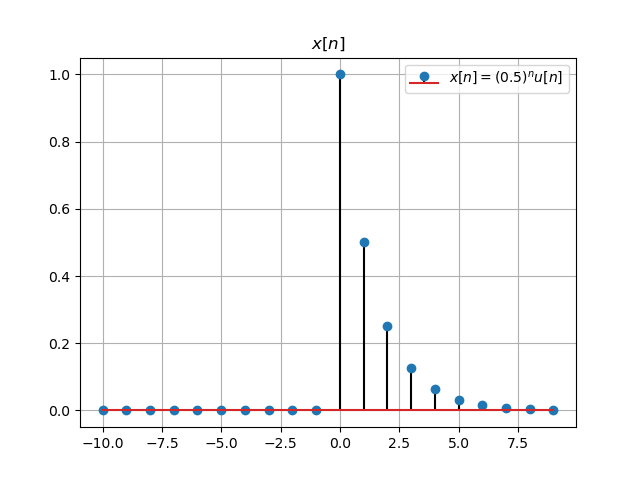
\includegraphics[width=\columnwidth]{graphs/x_n.png}
 \caption{$x[n] = \brak{\frac{1}{2}}^nu[n]$}
 \end{figure}
 
 \begin{figure}[!ht]
\centering
 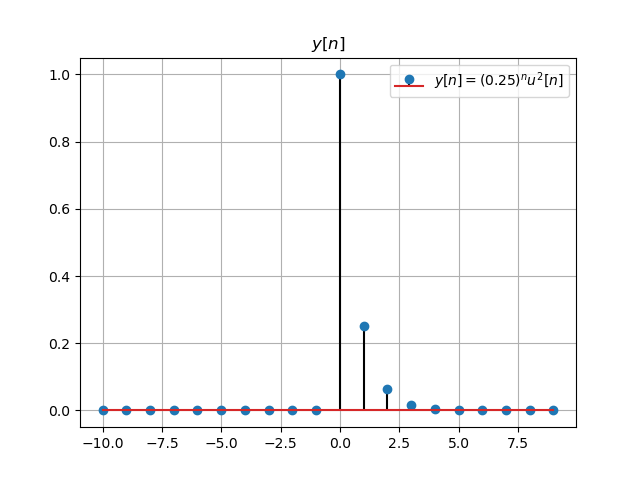
\includegraphics[width=\columnwidth]{graphs/y_n.png}
 \caption{$x[n] = \brak{\frac{1}{4}}^nu^2[n]$}
 \end{figure}
 
 \begin{figure}[!ht]
\centering
 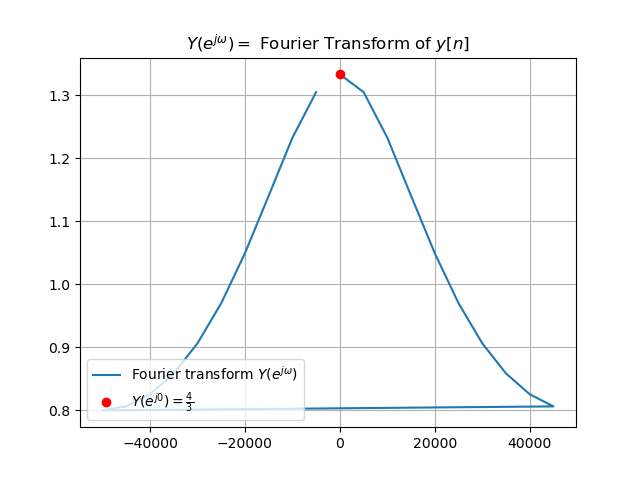
\includegraphics[width=\columnwidth]{graphs/fourier.png}
 \caption{$Y(e^{j\omega})$}
 \end{figure}
\end{document}
